\paragraph{DiffSound}

\textit{DiffSound} was presented in a paper, in 2022, that displays a novel text-to-sound generation framework that uses a text encoder, a \ac{VQ-VAE}, a decoder, and a vocoder. The framework takes text as input and outputs synthesized audio corresponding to the input text. The decoder, in particular, is a critical component of the framework, and the paper focuses on designing a suitable decoder, calling it \textit{DiffSound} \cite{yang_diffsound_2022}.

DiffSound is a diffusion decoder (Section \ref{sec:diffusion}) based on the discrete diffusion model. DiffSound predicts all Mel-Spectrogram tokens in one step and then refines the predicted tokens in the next step, resulting in better-predicted results after several steps. It not only produces better text-to-sound generation results compared to an \ac{AR} decoder, but it is also faster, with a generation speed five times faster than an \ac{AR} decoder.

The entire framework acts as this: First, the text is encoded into embeddings using a model like a transformer (Section \ref{sec:transformers}). Then, this representation conditions the generation of spectrogram embeddings using diffusion (the DiffSound model). These embeddings are then passed through the pretrain \ac{VQ-VAE} decoder to generate the spectrogram. The spectrogram runs through a vocoder (Section \ref{sec:vocoders}) to generate the waveform. In the original text, the vocoder used was the MelGAN (see Section \ref{sec:melgan}). This process can be seen in Figure \ref{fig:diffsound}.

\begin{figure}[ht]
    \centering
    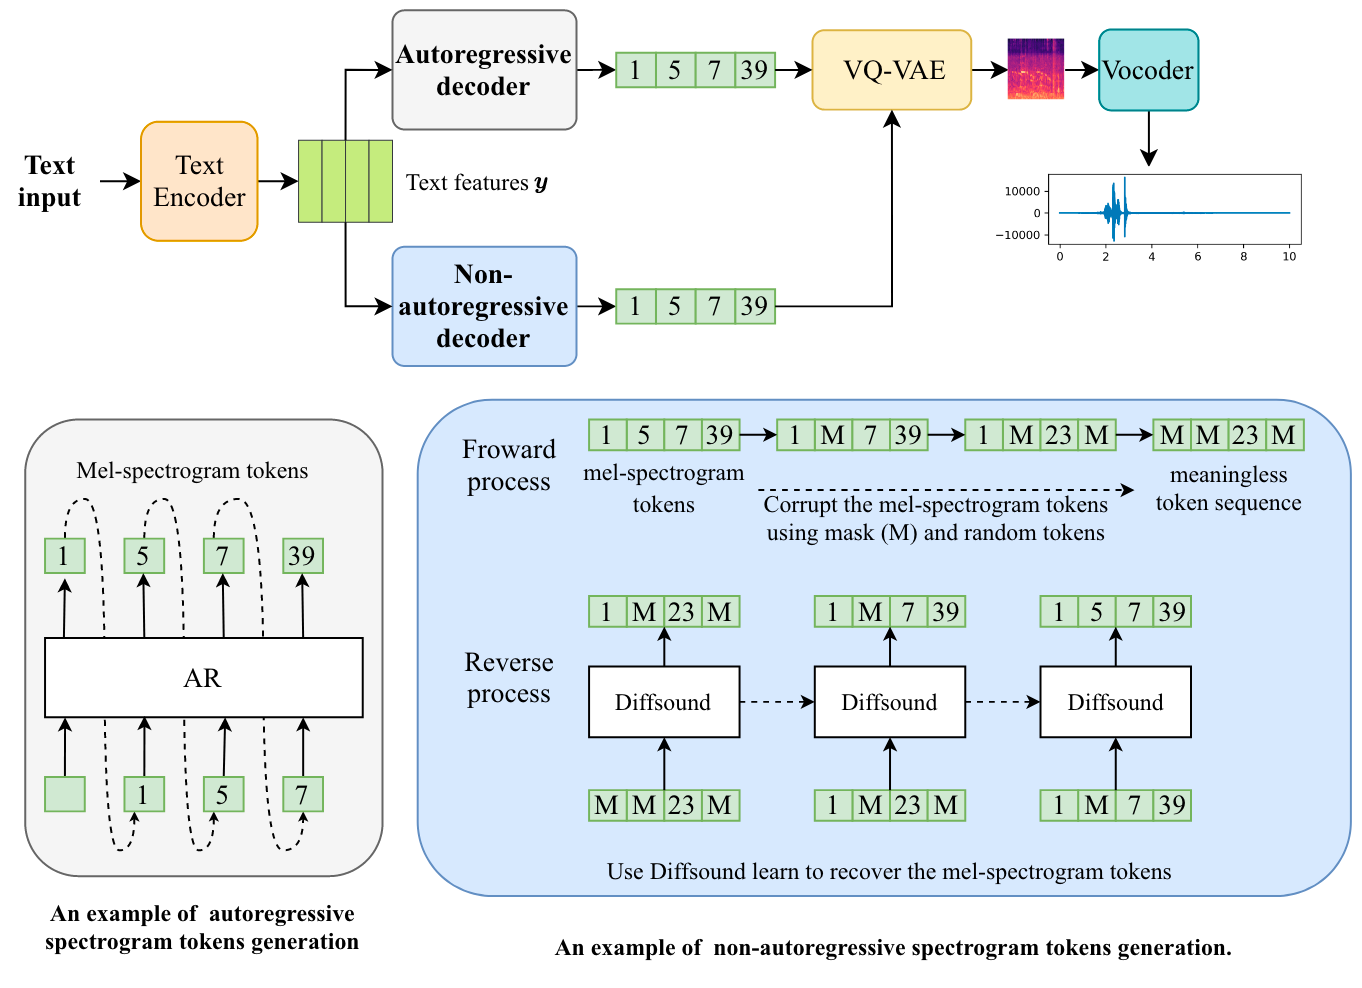
\includegraphics[width=\textwidth]{figures/2-sota/diffsound.png}
    \caption[DiffSound framework]{\textbf{DiffSound framework} --- This illustration was taken from the original paper. At the top, the general framework is present. Two decoders are present, but only one of them is used. The decoder results in a set of latent features. These features are passed to the decoder of the \ac{VQ-VAE} that generates a Mel-Spectrogram (the square with red and blue tones) that, through a vocoder, generates a sound. The two bottom images represent the two decoders. One is a \ac{DARN} (see Section \ref{sec:darn}), the other works with diffusion.}
    \label{fig:diffsound}
\end{figure}